\documentclass[a4paper]{article}

\usepackage{graphicx}

\begin{document}

\title{Lab Session 2: Resampling Statistics}

\author{Simon Harris \\
 	CE888: Data Science and Decision Making  \\
	University of Essex
}


\date{\today}

\maketitle


A Brief writeup on Lab 2 and getting stuck in with some of Python's Data Science toolkits.


\section{Setting Up}

\begin{enumerate}
\item \textbf{Did not} set up an Overleaf account as I'm familiar with \LaTeX and have tools to work with it
\item \textbf{Did} send an email to Ana with my GitHub username
\item \textbf{Did} download the slides and initial code, and upload to GitHub
\item \textbf{Did} download PyCharm, but am reluctant to use it to a great extent as I have tools I prefer
\end{enumerate}


\section{Data Visualisation}

Here I was pleased to be able to create a working \texttt{vehicles.py} and generate the scatter plot and histogram. This was admittedly mainly a case of copying and trimming the \texttt{salaries.py} code, but I made sure to take the time to understand it and learn about the libraries involved.

\begin{center}
   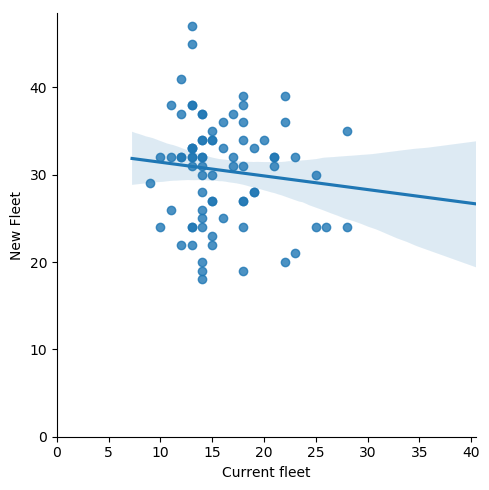
\includegraphics[scale=0.8]{veh_scatterplot.png}
   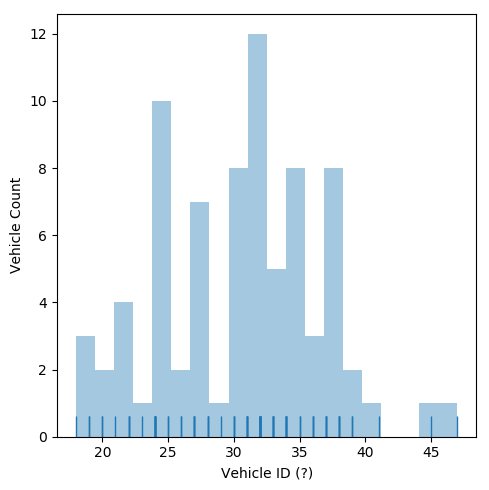
\includegraphics[scale=0.8]{veh_histogram.png}
\end{center}

\section{Exercise: Bootstrap 1}

This was somewhat more challenging, and it took me several hours to write very few lines of code! However, I was struck by how powerful those few lines are, and how much more complicated the solution would have been without libraries, in particular NumPy. In addition, I invested time in reviewing the lecture slides in order to understand the resampling algorithm, and also the libraries involved, which was a worthwhile endeavour.

\begin{center}
   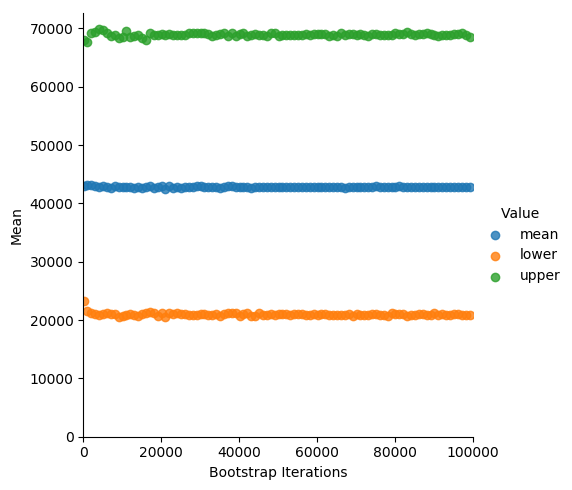
\includegraphics[scale=0.6]{bootstrap_confidence.png}
\end{center}

\section{Exercise: Bootstrap 2}

This was mainly just a case of calling my \texttt{bootstrap()} function from the previous exercise. It took me a while to find an overall mean for the dataset, but finally discovered that \texttt{df.mean().mean()} provides that.

I wasn't sure how many iterations and how large a sample size to use, so I chose arbitrary numbers, both fairly high but not high enough to take forever to run. Output was as follows:

\begin{verbatim}
Overall mean: 25.31279548574043
Old Lower: 19.313253012048193
Old Upper: 20.883734939759034
New Lower: 29.189873417721518
New Upper: 31.78481012658228
\end{verbatim}

I'm not sure how to decide whether these are "comparable". Given a 95\% confidence interval, the numbers for the old fleet are consistently below the overall mean, while the new fleet provides numbers consistently above it. Assuming that high numbers are good, one could conclude the new fleet to be better.

\end{document}